
\begin{frame}
    \frametitle{Operational layer}
    \begin{figure}
      \centering
      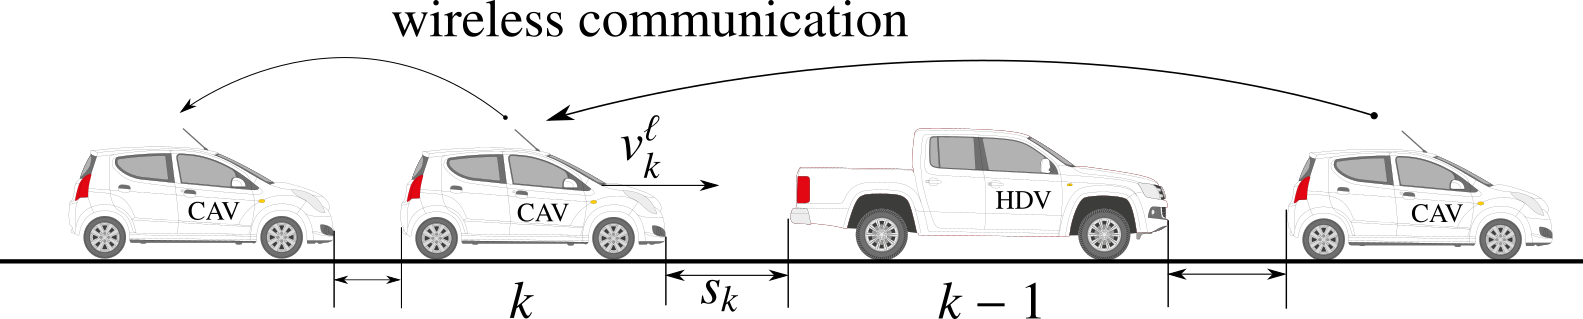
\includegraphics[width=0.7\linewidth]{fig_15_CAV_HDV_follow.png}
      \caption{Mixed traffic scenario}
    \end{figure}
    \begin{itemize}[<+->]
      \item Available measurements for a vehicle: 
      \begin{itemize}
       \item[\(s_k\)] Headway space 
       \item[\(v_k\)] Vehicle's speed
       \item[\(v_{k-1}\)] Leader's speed
      \end{itemize}
      \item Consideration of \structure{3rd order} linear dynamics. 
        \begin{equation*}
          x_i(s) = \left(\frac{1}{s}\right)\left(\frac{1}{s+b}\right)\left(\frac{1/T_e}{s+1/T_e}\right)
        \end{equation*}
    \end{itemize}
\end{frame}